\documentclass[conference]{IEEEtran}

\usepackage{cite}

\usepackage{graphicx}
\graphicspath{{fig/}}
\DeclareGraphicsExtensions{.pdf,.jpeg,.png}

\usepackage{algorithmic}

\usepackage{amsmath,amssymb}
\usepackage{algorithm}
\newtheorem{thm}{Theorem}
\newtheorem{prop}[thm]{Proposition}

\usepackage{multirow}

\usepackage{url}

% *** Do not adjust lengths that control margins, column widths, etc. ***
% *** Do not use packages that alter fonts (such as pslatex).         ***
% There should be no need to do such things with IEEEtran.cls V1.6 and later.
% (Unless specifically asked to do so by the journal or conference you plan
% to submit to, of course. )

% correct bad hyphenation here
\hyphenation{op-tical net-works semi-conduc-tor}


\begin{document}
%
% paper title
% can use linebreaks \\ within to get better formatting as desired
% Do not put math or special symbols in the title.
\title{MapReduce Reduced Support Vector Machine}


% author names and affiliations
% use a multiple column layout for up to three different
% affiliations
\author{
\IEEEauthorblockN{Wei-Chih Lai}
\IEEEauthorblockA{National Taiwan\\
University of\\
Science and Technology\\
Email: }
\and
\IEEEauthorblockN{Po-Han Huang}
\IEEEauthorblockA{National Taiwan\\
University of\\
Science and Technology\\
Email: }
\and
\IEEEauthorblockN{Yuh-Jye Lee}
\IEEEauthorblockA{National Taiwan\\
University of\\
Science and Technology\\
Email: \\
Telephone: }}

% conference papers do not typically use \thanks and this command
% is locked out in conference mode. If really needed, such as for
% the acknowledgment of grants, issue a \IEEEoverridecommandlockouts
% after \documentclass

% for over three affiliations, or if they all won't fit within the width
% of the page, use this alternative format:
% 
%\author{\IEEEauthorblockN{Michael Shell\IEEEauthorrefmark{1},
%Homer Simpson\IEEEauthorrefmark{2},
%James Kirk\IEEEauthorrefmark{3}, 
%Montgomery Scott\IEEEauthorrefmark{3} and
%Eldon Tyrell\IEEEauthorrefmark{4}}
%\IEEEauthorblockA{\IEEEauthorrefmark{1}School of Electrical and Computer Engineering\\
%Georgia Institute of Technology,
%Atlanta, Georgia 30332--0250\\ Email: see http://www.michaelshell.org/contact.html}
%\IEEEauthorblockA{\IEEEauthorrefmark{2}Twentieth Century Fox, Springfield, USA\\
%Email: homer@thesimpsons.com}
%\IEEEauthorblockA{\IEEEauthorrefmark{3}Starfleet Academy, San Francisco, California 96678-2391\\
%Telephone: (800) 555--1212, Fax: (888) 555--1212}
%\IEEEauthorblockA{\IEEEauthorrefmark{4}Tyrell Inc., 123 Replicant Street, Los Angeles, California 90210--4321}}




% use for special paper notices
%\IEEEspecialpapernotice{(Invited Paper)}




% make the title area
\maketitle

% As a general rule, do not put math, special symbols or citations
% in the abstract
\begin{abstract}
This paper propose a parallel algorithm named MapReduce Reduced Support Vector Machine(MRRSVM) which extend Reduced Support Vector Machine(RSVM), let non-liner SVM method able to handle super large scale data. There are many algorithms trying to extend non-linear SVM method. Most of them are based on SMO, shrinking technique or working set selection. Consider there are many training data, there is no necessary to enforce all instances joining in a single kernel. In this paper, we'll show that how to use a linear SVM to combine many small RSVM models. Our algorithm has two phase. The first phase is called "Map Phase", it splits dataset into many subsets and trains lots of RSVM models for each subset. The second phase is called "Reduce Phase", it treats each RSVM model as an expert for sub-data and use a linear SVM to vote their prediction in this phase. Combine these two phases, we'll get a binary classification for our big data. Finally, we apply non-linear SVM method on big data and speed up with parallel framework and reduced kernel trick. Experimental results show this algorithm is fast and fairly sharp for handling big data.
\end{abstract}

\smallskip
\noindent \textbf{Keywords.} RSVM, map reduce, super large scale big data

% For peer review papers, you can put extra information on the cover
% page as needed:
% \ifCLASSOPTIONpeerreview
% \begin{center} \bfseries EDICS Category: 3-BBND \end{center}
% \fi
%
% For peerreview papers, this IEEEtran command inserts a page break and
% creates the second title. It will be ignored for other modes.
\IEEEpeerreviewmaketitle

\section{Introduction}
% no \IEEEPARstarta
Data has became larger and larger due to data can be easily collected nowadays. People have to introduce new algorithms and structures to handle big data. The Support Vector Machine already showed good results on dealing with classic classification problem. There are several algorithms(\cite{platt1998sequential, joachims1999making, fan2005working, zhang2004solving, kivinen2004online, shalev2011pegasos, ouyang2010fast, fan2008liblinear}) are trying to apply SVM method on big data. For linear SVM, Liblinear\cite{fan2008liblinear} presents a well performed library combines a dual coordinate descent method and other technique to implement large-scale linear SVM. For non-linear SVM, SMO\cite{platt1998sequential} introduces an algorithm for solving the quadratic programming effectually. SMO-shrink\cite{joachims1999making} and SMO-wss2\cite{fan2005working} are extended SMO methods with selecting a good working set to reduce the size of quadratic programming problem. Those algorithms use lots of trick to squeeze instance and train a model like classic non-linear SVM.

Most algorithms are either linear method or approximate non-linear method because it is too difficult to build a full kernel for large data. By giving a data size $n$, having a linear combination solution of kernel function will require $n^2$ memory space. Since the data size goes millions upon millions, the $n^2$ space requirement is unreachable. Thankfully, we have RSVM that reduce the kernel size from $n^2$ to $nm$, which $m$ is way smaller than $n$. If we look inside RSVM, $m$ is actually $rn$, which $r$ is our ratio. So the kernel size of RSVM is actually $rn^2$. Like we just mention that the size of data grows fast, reduced kernel will finally meet the limit of memory space. So the main idea of our method is to split the super large scale data into small pieces. Noticed that even we use "small" here, the size of these pieces may be large but can be compute by RSVM.

Parallel is very popular nowadays, more and more algorithms are applied into parallel structure. Like \cite{graf2004parallel, collobert2002parallel} show that we can make SVM parallel itself. But in this paper, we focus on the map reduce structure which can be easily parallel because of every sub-set that we split in map phase are independent from each other. Due to the parallel structure and the small size of kernel, MRRSVM has a very good performance on speed as a non-linear method.

In Section~\ref{sec:RSVM}, we'll talk about RSVM which is the basic method of our algorithm. Then in Section~\ref{sec:MRRSVM}, we start to introduce the whole structure of our method. And in Section~\ref{sec:Experiments}, we are going to show performance of MRRSVM.

In summary, the key point of this method is:
\begin{enumerate}
  \item We split data into small pieces so that each we can make a RSVM model for it. This decision also make the whole architecture parallelable.
  \item Combine the non-linear RSVM models by using a linear SVM.
\end{enumerate}

\section{RSVM}
\label{sec:RSVM}
The Reduced Support Vector Machine(RSVM) aims to generate a non-linear separating hyperplane of a large dataset by keeping a little subset and throwing remainder. For data matrix $A \in R^{m\times n}$, the standard SVM will build kernel matrix with $K(A, A') \in R^{m\times m}$. Once the dataset has a lot of instance, standard kernel matrix will makes the computer running out of memory quickly. To avoid computing difficulty, RSVM uses a small subset, $\bar{A}$, which is randomly selected from the original dataset to build kernel. After cutting the problem size, kernel matrix $K(A, \bar{A}')$ is in $R^{m\times \bar{m}}$ and $\bar{m}$ is $m$ multiplied by reduction ratio (typically less than 0.1). Computational results indicate that this data-reduction approach can work fairly well and reduced dataset is all needed in generating the final non-linear separating hyperplane. This is very important for handling the large dataset. The standard SVM can handle because building huge full kernel matrix for large dataset is impossible. With RSVM, we can use a reduced kernel matrix to generate a separating hyperplane instead of full kernel matrix. However, RSVM only reduces column number of kernel matrix. If the dataset has extreme number of instance, then the computing difficulty will back.

\begin{figure*}[t]
	\centering
	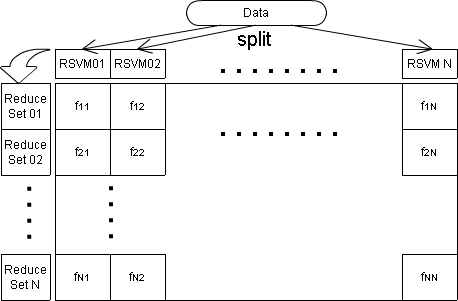
\includegraphics[width=0.6\linewidth]{structure.png}
	\caption{MRRSVM structure}
	\vskip 10 pt
	\label{fig:structure}
\end{figure*}

\section{MRRSVM}
\label{sec:MRRSVM}
To deal with super large scale data, we now introducing our algorithm. Map Reduced Reduced Support Vector Machine(MRRSVM) is an algorithm which can be paralleled due to its split structure. In this paper, to simplify the question, we focus on binary classification.

\subsection{Training}
Fig.~\ref{fig:structure} shows the whole structure of our algorithm. The first part which is called "Map Phase". In the figure is the part that data split into little pieces and each is trained by a RSVM. And the second part is "Reduce Phase". In this phase, we put all reduce sets which picked by our RSVMs as our new row element. This element will be combined as the new feature for our last linear SVM training with function $f_{ij}$ which we will define later.
The whole structure has only one propose, making non-linear SVM possible to train a super-large data. But in this propose, we can also have another advantage which is shorter training time. With building smaller kernels rather than one giant kernel, we can have a parallelable and quicker algorithm.

\subsubsection{Map Phase : Generate experts for local data}
In map phase, we're trying to make the super large-scale data fit in the kernel because we don't have infinite memory in real world. While using RSVM, we've already fix some problems that big kernel bring to us. But still, kernel has its own limit. Instead of changing kernel, we split data into small pieces. So that we can make a lot of fitting kernels to get RSVM models that we want for prediction.

Original data are split into $n$ subsets. Each data subset are going to train a model by RSVM with a reduced subset distributively. We also make parallel this part that all RSVM models can compute in the same time because every subset is independent. After having these $n$ RSVM models independently, models will be combined and concluded in out next phase, Reduce Phase.

In this phase, we have to make sure that our small RSVM models which make from split data can as approach the SVM model made by full data as possible. First, we let the data split in the same distribution as the original one. 

\subsubsection{Reduce Phase : Learning from experts’ estimation}
In reduce phase, combining the results of small RVSMs is what we have to do. For this purpose, we design a structure that use a linear SVM to train a final model which input data is the things we receive from RSVMs. We collect all the instances from those $n$ reduced subset we created in map phase. And next, we encode each of those instances as an $n$-dimensional vector by its estimated values from predicting them on RSVM models. To build this new instance, we create a function $f_{ij}$ which $i$ means the reduced set got from each split subset and $j$ means which RSVM model is used to get our estimated values. We now defining this function as:

\vspace{0.4cm}
$f_{ij}=K(ReduceSet_i,model_j.RS) \times model_j.w-model_j.b$
\vspace{0cm}

This function is used to estimate the label in RSVM. The term $K(ReduceSet_i,model_j.RS)$ is to compute the kernel value between reduce set $i$ and model $j$. Here the $model_j.RS$ is the reduce set we selected while creating RSVM model. These reduce set are used to build kernel with other set of instance to have the kernel value between other set and the model. So it is actually a representation of full set used by the model. Notice that we remain the same data size of all reduced subsets with the $n$-dimensional features described by those $n$ RSVM models. Finally, we will get the same reduce set size which can represent the whole data set. We'll use these reduce set the get our estimation with our RSVM models. Once we have these estimated values, we can apply the linear SVM to conclude the final MRRSVM model by compressing the data. The detail of our algorithm is shown in Algorithm \ref{algo:train}.
  
In this definition, each RSVM can be seen as an expert for its own set and each reduced sets stand for the point of view that expert specify in. What we do next is to let every expert(RSVM) to estimate all reduced sets, letting us get a table full of estimate number. Then we use it as new input data for linear SVM. While using estimate numbers produce by RSVMs as training data, we actually let the linear SVM weighting our experts. 

Because every small RSVM only learn things from one subset, it is actually a local expert. We can not make sure that a local expert will be doing well in global field. Due to these, subset choosing maybe a very important issue in this method.

\begin{algorithm}
\begin{algorithmic}
\caption{MapReduce RSVM train}
\label{algo:train}
\REQUIRE The big dataset $A$.
\ENSURE RSVM model $\{model_i\}^n_{i=1}$, the reduced set of each subset $\{\tilde{A_i}\}$, the linear SSVM model $\{model_{final}\}$ with new features generated by $\{model_i\}^n_{i=1}$
\begin{enumerate}
  \item Split $A$ into $n$ subsets and their associated reduced sets: $\{A_i\}^n_{i=1}$ and $\{\tilde{A_i}\}^n_{i=1}$
  \item Learn the RSVM $model_i$ for each subset $A_i$ with its reduced set $\tilde{A_i}$
  \item Generate a new representation $B\in\mathbb{R}^{(\Sigma\tilde{\ell_i})\times n}$ for the reduced subsets and the $j$th row of $B$ is represented as follow:\\
  $\mathbf{x}^{new}_j=[model_1(\mathbf{x}_j),model_2(\mathbf{x}_j),\dots,model_n(\mathbf{x}_j)]^T\in \mathbb{R}^n$ for $\mathbf{x}_j \in \{\tilde{A_i}\}^n_{i=1}$
  \item Learn the linear SSVM model with $B$:\\
  $model_{final} \gets linear\_$SVM$\_train(B)$
  \item Return $\{model_i\}^n_{i=1}$, $\{\tilde{A_i}\}^n_{i=1}$, and $model_{final}$
\end{enumerate}
\end{algorithmic}
\end{algorithm}

\subsection{Predicting}
Predict is also an important problem in binary classification. To efficiently predict label is the critical issue in this part. Thankfully, prediction doesn't need to change the model so that we don't have to worry about if each split subset have too few instances or the label in each split subset is unbalance. In this part, we use the same idea while we train. Map the test data into little pieces which allow us the compute paralleled and build smaller kernel to save more time. And then encode them into $n$-dimensional vector using $n$ RSVM models estimated values, these RSVM models are what we learned in training part. Next we Reduce these results into a linear SVM which is the final model we learned before. The detail for prediction is shown in Algorithm \ref{algo:predict}.

\begin{algorithm}
\begin{algorithmic}
\caption{MapReduce RSVM predict}
\label{algo:predict}
\REQUIRE A testing instance $\mathbf{x}_t$, $\{model_i\}^n_{i=1}$, and $model_{final}$
\ENSURE Predicted label
\begin{enumerate}
  \item Generate the new representation for the testing instance $\mathbf{x}_t$:\\
  $\mathbf{x}^{new}_t = [model_1(\mathbf{x}_j),model_2(\mathbf{x}_j),\dots,model_n(\mathbf{x}_j)]^T\in \mathbb{R}^n$
  \item Predicted label $\gets$ sign$(model_{final}(\mathbf{x}^{new}_t))$
\end{enumerate}
\end{algorithmic}
\end{algorithm}


\section{Experiments}
\label{sec:Experiments}
In this section, we focus on the general of our method and the strength of our classification. Also we're interesting in the performance for each RSVM models and the difference between those RSVM models and final linear SVM model. First, we use a toy problem called checkerboard to proof that our method remain the same ability as RSVM. Instead of using the original checkerboard which size is 2,000, we create a new checkerboard size 1,000,000. Second, we're trying to approach the well turned model as possible as we can. For this propose, we implement uniform design to choose the parameters for us. Third, we design an experimental that all methods only use the default parameters while training. This experiment is to show the general of our tool. Even through there is uniform design, you can't expect every user waiting for such a long time for the well tuned model. Especially for those hard turned dataset like covertype. Since we compare our method with libsvm and RSVM, we use both default parameters. So that we get two pair of parameters and three method to test, we'll have total six results for each dataset.  Notice that our method is fast and parallel, waiting time for well tuned model will effectively decrease. But making things easier doesn't mean that this thing will become cost free. Still, tuning is a hard work and don't know where to ended.

\subsection{Experiment Environment}

\subsection{Preprocessing}
The preprocessing for each dataset is the same. First, normalizing each attribute column between -1 and 1. Second, calculating the frequent of classes. Final, split dataset to several files with same size. Also, we make sure that each subset will remain the same proportion of labels. We let each training subset not more than 25,000 instances and for each testing set not more than a specified size of instances. These bounds are to going to limit our kernel size but not to lose too much information after splitting. 

\subsection{Experiment Setting}
While training RSVM model in map phase, we need to choose the value of cost, gamma and ratio. And for final linear SVM, we need to decide the value of cost. Usually, ratio is setted to 0.1. The rest three parameters will choose by uniform design\cite{fang2000uniform} which is also introduced in Section \ref{sec:RSVM}.

\subsection{Experiment Results}
\subsubsection{Checkerboard}
A checkerboard dataset is to show the ability of a non-linear SVM. To proof that we remain the feature of RSVM and have the ability to handle large scale data, we use a data with size $1,000,000$ for training and $2,000$ for testing. Fig.(ref) shows the result of the test data. Even those it is a toy problem, it still represents the power of non-linear method.

\subsubsection{Well Tune Model Experiment}
In this part, we use uniform design to find the approach of the best tune models for some datasets. Including svmguide1, w3a, a9a, ijcnn1, zero1 and covtype. 

Svmguide1 is a dataset size is 3,089 and has a test set which size is 4,000.

\begin{table*}[!t]
% increase table row spacing, adjust to taste
\renewcommand{\arraystretch}{1.3}
% if using array.sty, it might be a good idea to tweak the value of
%\extrarowheight as needed to properly center the text within the cells
\caption{Result of well tuned model}
\label{table_example}
\centering
\begin{tabular}{|c|c|c|c|c|c|c|c|c|c|}
\hline
DataSet & SFW & SFW & MSFW & MSII-W & SMO- & SMO- & SMO- & SMO-& MapReduce\\
& 1 epo. & 2 epo. & 1 epo. & 2 epo. & L2 & L1 & shrink & wss2 & RSVM\\
\hline
\multirow{2}{*}{svmguide1} & 
96.85 & 96.98 & 97.00 & 97.00 & 97.00 & 97.00 & 97.00 & 97.00 & 97.05\\
\cline{2-10}
& 0.30 & 0.86 & & & & & & &\\
\hline
\end{tabular}
\end{table*}

\subsubsection{General Experiment}
Subsubsection text here.

\subsubsection{Discover During Experiment}
Subsubsection text here.


%\begin{figure}
%	\centering
%	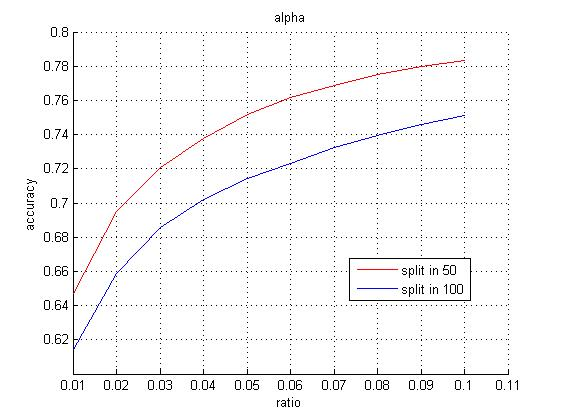
\includegraphics[width=\linewidth]{alpha1.jpg}
%	\caption{alpha1}
%	\vskip 10 pt
%	\label{fig:alpha1}
%\end{figure}
%\begin{figure}
%	\centering
%	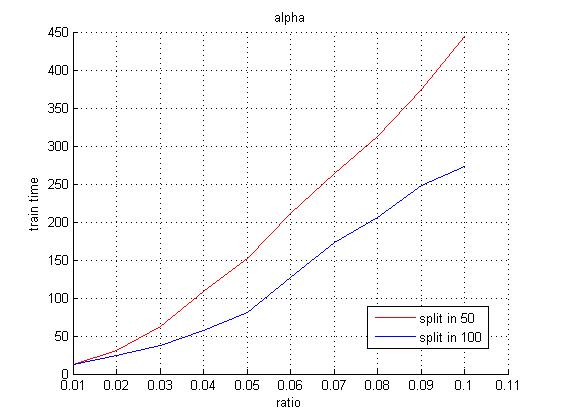
\includegraphics[width=\linewidth]{alpha2.jpg}
%	\caption{alpha2}
%	\vskip 10 pt
%	\label{fig:alpha2}
%\end{figure}
%\begin{figure}
%	\centering
%	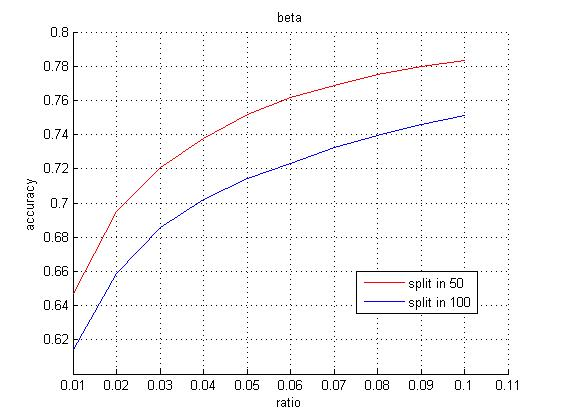
\includegraphics[width=\linewidth]{beta1.jpg}
%	\caption{beta1}
%	\vskip 10 pt
%	\label{fig:beta1}
%\end{figure}
%\begin{figure}
%	\centering
%	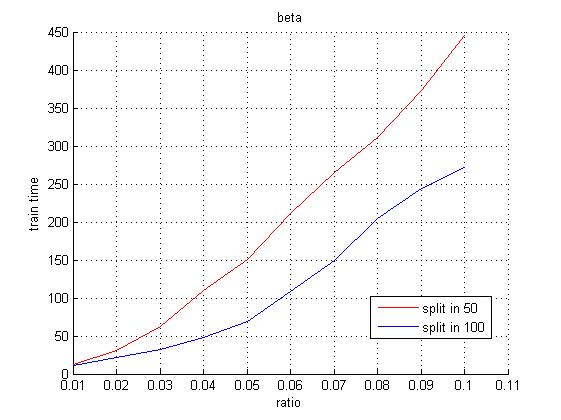
\includegraphics[width=\linewidth]{beta2.jpg}
%	\caption{beta2}
%	\vskip 10 pt
%	\label{fig:beta2}
%\end{figure}
%\begin{figure}
%	\centering
%	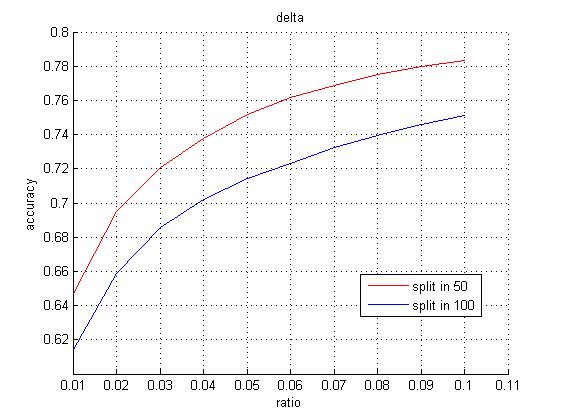
\includegraphics[width=\linewidth]{delta1.jpg}
%	\caption{delta1}
%	\vskip 10 pt
%	\label{fig:delta1}
%\end{figure}
%\begin{figure}
%	\centering
%	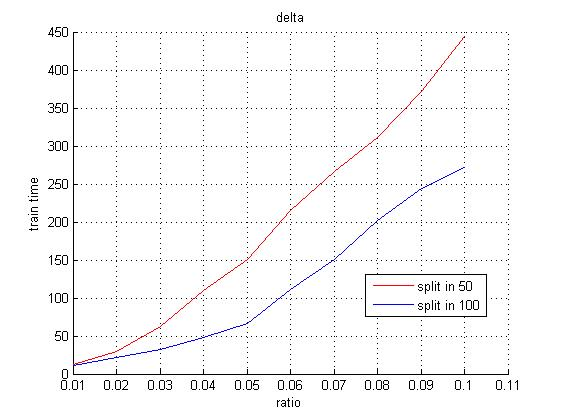
\includegraphics[width=\linewidth]{delta2.jpg}
%	\caption{delta2}
%	\vskip 10 pt
%	\label{fig:delta2}
%\end{figure}
%\begin{figure}
%	\centering
%	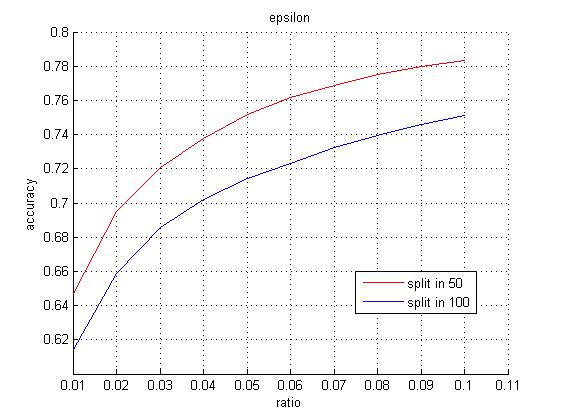
\includegraphics[width=\linewidth]{epsilon1.jpg}
%	\caption{epsilon1}
%	\vskip 10 pt
%	\label{fig:epsilon1}
%\end{figure}
%\begin{figure}
%	\centering
%	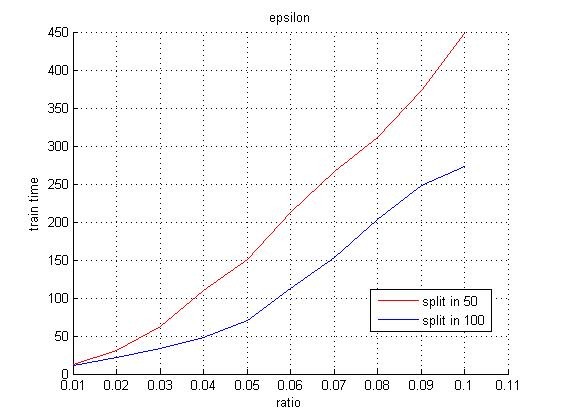
\includegraphics[width=\linewidth]{epsilon2.jpg}
%	\caption{epsilon2}
%	\vskip 10 pt
%	\label{fig:epsilon2}
%\end{figure}
%\begin{figure}
%	\centering
%	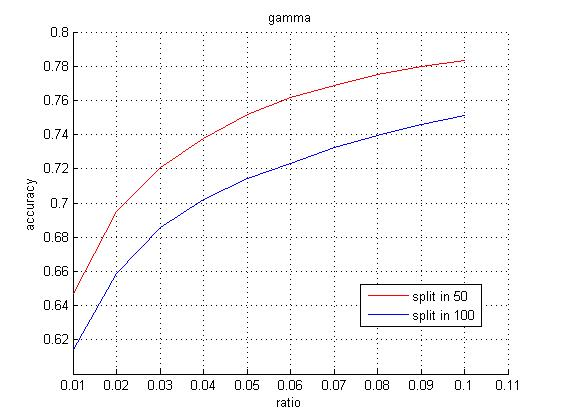
\includegraphics[width=\linewidth]{gamma1.jpg}
%	\caption{gamma1}
%	\vskip 10 pt
%	\label{fig:gamma1}
%\end{figure}
%\begin{figure}
%	\centering
%	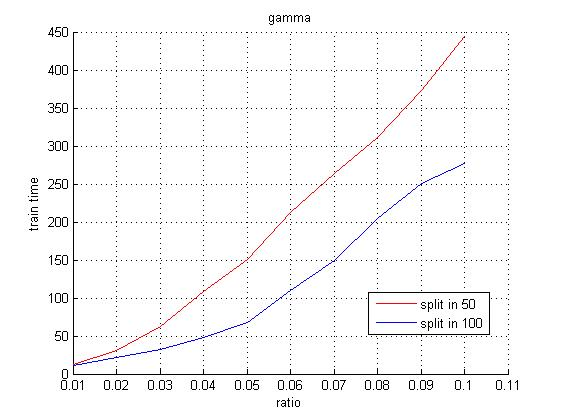
\includegraphics[width=\linewidth]{gamma2.jpg}
%	\caption{gamma2}
%	\vskip 10 pt
%	\label{fig:gamma2}
%\end{figure}
%\begin{figure}
%	\centering
%	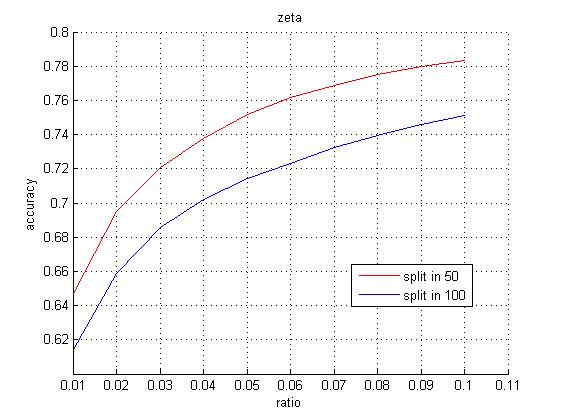
\includegraphics[width=\linewidth]{zeta1.jpg}
%	\caption{zeta1}
%	\vskip 10 pt
%	\label{fig:zeta1}
%\end{figure}
%\begin{figure}
%	\centering
%	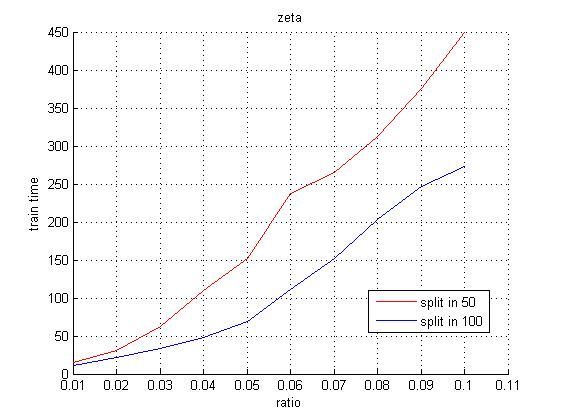
\includegraphics[width=\linewidth]{zeta2.jpg}
%	\caption{zeta2}
%	\vskip 10 pt
%	\label{fig:zeta2}
%\end{figure}


% An example of a floating figure using the graphicx package.
% Note that \label must occur AFTER (or within) \caption.
% For figures, \caption should occur after the \includegraphics.
% Note that IEEEtran v1.7 and later has special internal code that
% is designed to preserve the operation of \label within \caption
% even when the captionsoff option is in effect. However, because
% of issues like this, it may be the safest practice to put all your
% \label just after \caption rather than within \caption{}.
%
% Reminder: the "draftcls" or "draftclsnofoot", not "draft", class
% option should be used if it is desired that the figures are to be
% displayed while in draft mode.
%
%\begin{figure}[!t]
%\centering
%\includegraphics[width=2.5in]{myfigure}
% where an .eps filename suffix will be assumed under latex, 
% and a .pdf suffix will be assumed for pdflatex; or what has been declared
% via \DeclareGraphicsExtensions.
%\caption{Simulation Results.}
%\label{fig_sim}
%\end{figure}

% Note that IEEE typically puts floats only at the top, even when this
% results in a large percentage of a column being occupied by floats.


% An example of a double column floating figure using two subfigures.
% (The subfig.sty package must be loaded for this to work.)
% The subfigure \label commands are set within each subfloat command,
% and the \label for the overall figure must come after \caption.
% \hfil is used as a separator to get equal spacing.
% Watch out that the combined width of all the subfigures on a 
% line do not exceed the text width or a line break will occur.
%
%\begin{figure*}[!t]
%\centering
%\subfloat[Case I]{\includegraphics[width=2.5in]{box}%
%\label{fig_first_case}}
%\hfil
%\subfloat[Case II]{\includegraphics[width=2.5in]{box}%
%\label{fig_second_case}}
%\caption{Simulation results.}
%\label{fig_sim}
%\end{figure*}
%
% Note that often IEEE papers with subfigures do not employ subfigure
% captions (using the optional argument to \subfloat[]), but instead will
% reference/describe all of them (a), (b), etc., within the main caption.


% An example of a floating table. Note that, for IEEE style tables, the 
% \caption command should come BEFORE the table. Table text will default to
% \footnotesize as IEEE normally uses this smaller font for tables.
% The \label must come after \caption as always.
%
%\begin{table}[!t]
%% increase table row spacing, adjust to taste
%\renewcommand{\arraystretch}{1.3}
% if using array.sty, it might be a good idea to tweak the value of
% \extrarowheight as needed to properly center the text within the cells
%\caption{An Example of a Table}
%\label{table_example}
%\centering
%% Some packages, such as MDW tools, offer better commands for making tables
%% than the plain LaTeX2e tabular which is used here.
%\begin{tabular}{|c||c|}
%\hline
%One & Two\\
%\hline
%Three & Four\\
%\hline
%\end{tabular}
%\end{table}


% Note that IEEE does not put floats in the very first column - or typically
% anywhere on the first page for that matter. Also, in-text middle ("here")
% positioning is not used. Most IEEE journals/conferences use top floats
% exclusively. Note that, LaTeX2e, unlike IEEE journals/conferences, places
% footnotes above bottom floats. This can be corrected via the \fnbelowfloat
% command of the stfloats package.



\section{Conclusion}
The conclusion goes here.




% conference papers do not normally have an appendix


% use section* for acknowledgement
\section*{Acknowledgment}


The authors would like to thank...





% trigger a \newpage just before the given reference
% number - used to balance the columns on the last page
% adjust value as needed - may need to be readjusted if
% the document is modified later
%\IEEEtriggeratref{8}
% The "triggered" command can be changed if desired:
%\IEEEtriggercmd{\enlargethispage{-5in}}

% references section

% can use a bibliography generated by BibTeX as a .bbl file
% BibTeX documentation can be easily obtained at:
% http://www.ctan.org/tex-archive/biblio/bibtex/contrib/doc/
% The IEEEtran BibTeX style support page is at:
% http://www.michaelshell.org/tex/ieeetran/bibtex/
%\bibliographystyle{IEEEtran}
% argument is your BibTeX string definitions and bibliography database(s)
%\bibliography{IEEEabrv,../bib/paper}
%
% <OR> manually copy in the resultant .bbl file
% set second argument of \begin to the number of references
% (used to reserve space for the reference number labels box)
%\begin{thebibliography}{1}

%\bibitem{IEEEhowto:kopka}
%H.~Kopka and P.~W. Daly, \emph{A Guide to \LaTeX}, 3rd~ed.\hskip 1em plus
% 0.5em minus 0.4em\relax Harlow, England: Addison-Wesley, 1999.


%\end{thebibliography}

\bibliographystyle{IEEEtran}
\bibliography{IEEEabrv,ref}

% that's all folks
\end{document}